\documentclass[10pt]{article}


\usepackage{graphicx}
\usepackage{tikz}
\graphicspath{{./img/}}

\usepackage{algorithm}
\usepackage{algorithmic}

% Math
\usepackage{amsmath, amssymb}







\begin{document}
\begin{titlepage}
    \vspace*{3cm}
    
    \centering
    {\Huge\bfseries\scshape
    Carcassonne}

    \vspace{1cm}

    \Large
    Mohammed Dlimi, Ismail Hatti, Ossama Aidoun


    \vfill

    Projet de programmation de langage C \\
    Département Informatique \\
    S6 - Année 2023/2024

    \vspace{1cm}

    \begin{figure}[hbt] 
        \centering
        
\includegraphics[width=0.5\textwidth]{images/logo_em.jpg}
    \end{figure}
    
    \vspace{3cm}
\end{titlepage}

\renewcommand{\contentsname}{Tables des matières}

\tableofcontents 

\section{Introduction}

\begin{figure}[h]
    \centering
    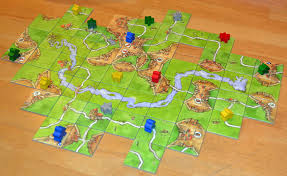
\includegraphics[width=0.5\textwidth]{images/Carcassonne.jpeg}
    \caption{(image tirée du site www.theboardgamefamily.com)}
    \label{fig:enter-label}
\end{figure}
%### Carcassonne : Un Classique Moderne des Jeux de Société

\subsection{Présentation générale du projet}
Carcassonne est un jeu de société moderne qui a su captiver l'imagination des joueurs depuis sa sortie en 2000. Créé par Klaus-Jürgen Wrede et édité par Hans im Glück, ce jeu tire son nom de la célèbre cité médiévale fortifiée située dans le sud de la France. Avec ses règles simples mais stratégiquement profondes, Carcassonne est devenu un pilier incontournable des soirées jeux de société à travers le monde.

\subsection{Principe du Jeu}
Le principe de Carcassonne est de construire un paysage médiéval en posant des tuiles représentant des villes, des routes, des champs et des abbayes. Chaque joueur dispose de partisans, aussi appelés meeples, qu'ils peuvent placer sur les tuiles pour revendiquer des territoires et marquer des points. Le but est d'avoir le plus de points à la fin de la partie.

\subsection{Déroulement d'une Partie}
\begin{itemize}
    \item \textbf{Mise en Place} : Au début de la partie, une tuile de départ est placée au centre de la table. Les autres tuiles sont mélangées et placées en piles face cachée.
    \item \textbf{Tour de Jeu} : À son tour, un joueur pioche une tuile et doit la placer de manière à ce qu'elle se connecte logiquement aux tuiles déjà en jeu. Par exemple, une route doit se connecter à une autre route, une ville à une autre ville, etc.
    \item \textbf{Placement des Meeples} : Après avoir placé une tuile, le joueur peut choisir de placer un meeple sur l'un des éléments de la tuile (ville, route, abbaye ou champ). Le meeple reste sur cette tuile jusqu'à ce que l'élément soit complété (comme la clôture d'une ville ou la fin d'une route).
    \item \textbf{Comptage des Points} : Une fois qu'un élément est complété, le joueur récupère son meeple et marque des points selon la taille de l'élément. Les champs, quant à eux, sont évalués à la fin de la partie.
\end{itemize}




%#### Stratégies et Complexité
Bien que Carcassonne soit facile à apprendre, il offre une profondeur stratégique surprenante. Les joueurs doivent constamment évaluer les risques et les récompenses de chaque placement de tuile et de meeple. Doivent-ils essayer de compléter leurs propres villes ou routes, ou gêner les autres joueurs ? Le positionnement des champs peut également être crucial, offrant des points supplémentaires en fin de partie pour chaque ville adjacente.
\subsection{Arborescence du dépot}
\begin{itemize}
    \item build :    \%contient tous les fichiers objets
    \item install
    \begin{itemize}
        \item all tests : \% l'exécutable des tests.
        \item server    : \% l'exécutable de la partie de jeu
        \item libplayer1.so : \% la bibliothèque dynamique du premier joueur.
        \item libplayer2.so : \% la bibliothèque dynamique du deuxième joueur.      
    \end{itemize}
    \item src : \% contient les codes sources sans les tests
    \begin{itemize}
        \item players : \% contient les deux fichiers sources des deux joueurs.
        \begin{itemize}
            \item player1.c 
            \item player2.c
        \end{itemize}
        \item les fichiers sources et d'en-têtes comme board.c board.h
    \end{itemize}
    \item tst : \% contient tous les fichiers sources pour les tests
    \item Makefile : \% compile l'ensemble des fichiers ainsi que les bibliothèques dynamiques des joueurs .
    \item README : \% contient des lignes d'explication afin de pouvoir compiler et exécuter les codes .
    \item .gitignore :  \% ignore les fichiers temporaires par git.
\end{itemize}
\subsection{Architecture du code}
Le projet est composé d’un ensemble de fichiers rédigés en langage de programmation C. Il comprend trois catégories de fichiers : les fichiers sources portant
l’extension ”.c” ,les fichiers d’en-tête portant l’extension ”.h” et les bibliothèques dynamiques poartant l'extension ".so". Les fichiers sources sont dédiés à la mise en œuvre du code, tandis que les fichiers d’en-tête servent à stocker les fonctions écrites dans les fichiers sources. Ils définissent également des variables globales en utilisant define, ainsi qu'un tableau \textbf{TILES\_TYPE} à l’aide de ”extern”.Chaque fichier fait les ”include” nécessaire pour la compilation. Nous avons adopté un fichier Makefile qui crée un fichier objet pour chaque fichier source, puis compile l’ensemble des fichiers en deux exécutables nommés ”server” pour les fichiers sources dans le répertoire \textbf{src} et ”alltests” pour les tests dans le répertoire \textbf{tst}. le fichier Makefile est censé aussi de compliler les bibliothèques dynamiques des joueurs. Ces dernières ainsi que les deux exécutables sont placés dans le répetoire \textbf{install}. En ce qui concerne les tests, nous avons utilisé des instructions ”printf” et ”assert” pour effectuer autant de tests que possible pour chaque fonction, en prenant en compte des cas extrêmes,de plus on a utilisé l'outil de développement logiciel \textbf{gcov} pour mesurer la couverture des tests.
voici le graphe de dépendances des fichiers sources situés dans la racine du répertoire \textbf{src}:
\begin{figure}[h]
    \centering
    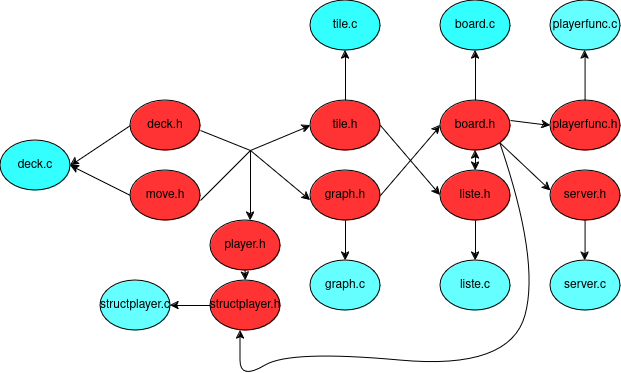
\includegraphics[width=0.9\textwidth]{images/Carcasonne.drawio(1).png}
    \caption{le graphe de dépendances des fichiers de \textbf{src} }
    \label{graphe de dépendaces}
\end{figure}
\section{Plateau de jeu}
\subsection{Tuiles}
En observant la forme des tuiles de Carcassonne,on peut remarquer que chaque tuile est caractériser par 13 positions Comme l’illustre la figure \ref{positions tuiles}, 3 sur chaque côté et une au centre:

\begin{figure}[h]
     \begin{minipage}{0.48\textwidth}
    \centering
    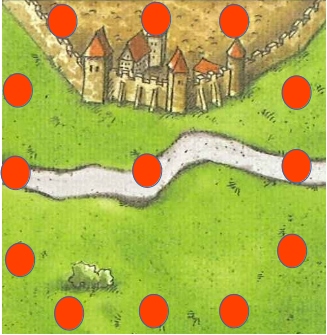
\includegraphics[width=0.6\textwidth,height=3.5cm]{images/tile1.png}
    \end{minipage}\hfill
    \begin{minipage}{0.48\textwidth}
    \centering
    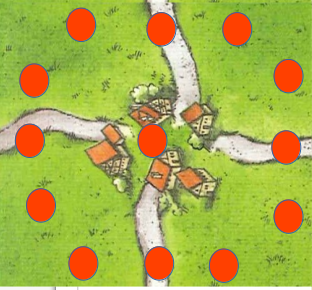
\includegraphics[width=0.6\textwidth,height=3.5cm]{images/tile2.png}
    \end{minipage}
    \caption{Les positions qui caractérisent les tuiles de Carcassonne}
    \label{positions tuiles}
\end{figure}
cela nous donne une idée pour définir une structure des tuiles. Comme le jeu contient un nombre fini d'objets (ville,route,champ,abbaye),on peut donc associer  à chaque objet une couleur. Par exemple,marron pour les villes,vert pour les champs,gris pour les routes...etc. Finalement toute tuile peut être représenté par la structure \textit{struct tile\_t} suivante:

\[
\text{struct tile\_t} \left\{
\begin{array}{l}
\text{t} \quad \rightarrow \quad \text{tableau d'entiers de taille 13}\\
\text{c} \quad \rightarrow \quad \text{tableau de couleurs de taille 13}\\
\end{array}
\right.
\]

\subsection{Pioche}
La pioche sera représentée par un type abstrait de données \textit{struct deck\_t}, dont l'implémentation dans le fichier deck.c contient trois champs:
\begin{itemize}
    \item deck qui un pointeur pointant sur les tuiles et qui sera alloué dynamiquement.
    \item size qui indique le nombre de tuiles stockées.
    \item capacity qui indique la taille de la mamoire allouée.
\end{itemize}
\[
\text{struct deck\_t} \left\{
\begin{array}{l}
\text{deck} \quad \rightarrow \quad \text{un poiteur pointant sur un tableau de tuiles }\\
\text{size} \quad \rightarrow \quad \text{entier}\\
\text{capacity} \quad \rightarrow \quad \text{entier}\\
\end{array}
\right.
\]
\subsection{Plateau}
\subsubsection{Plateau est un TAD }
Le plateau peut être implémenté de diverses façons, telles qu'une matrice ou une liste chaînée. Par conséquent, il est essentiel que la structure du Plateau soit un type abstrait de données, ce qui permet de rendre son implémentation plus flexible et indépendante du reste du code. \\
Pour représenter le plateau, une méthode simple consiste à utiliser une matrice de taille 2N, où N correspond au nombre total de tuiles. Cette approche offre plusieurs avantages, notamment un accès aux éléments du plateau en temps constant. Toutefois, cette méthode présente un inconvénient majeur : sa complexité en espace est de O($N^2$), ce qui est très coûteux en termes de mémoire.

Une deuxième méthode consiste à représenter le plateau par un tableau de taille N avec N le nombre de tuiles totales. Bien qu'il soit évident que cette méthode augmente la complexité en temps de certaines primitives, elle garantit une complexité linéaire en termes d'espace. Comme nous le verrons par la suite, la plupart des algorithmes associés à cette méthode sont linéaires, rendant cette approche plus envisageable.

Désormais, nous allons détailler la conception de la deuxième méthode.
\subsubsection{Tuiles dans le plateau}
\subsubsection*{Stockage des tuiles}
Stocker l'intégralité des tuiles dans le plateau augmenterait considérablement la complexité en espace. De plus, le nombre de tuiles différentes est fini. Par conséquent, nous pouvons stocker toutes les tuiles possibles dans un tableau \textbf{TILES\_TYPE}. Ainsi, nous pourrons stocker les tuiles dans le plateau en utilisant uniquement leurs indices dans \textbf{TILES\_TYPE}.
\subsubsection*{Rotation des tuiles}
Pendant la partie, la rotation des tuiles est autorisée. Il est donc nécessaire de savoir comment chaque tuile a été orientée. Pour ce faire, nous ajoutons un deuxième champ qui détermine l'orientation de la tuile sur le plateau.
\subsubsection*{Coordonnées et voisines d'une tuile}
Pour poser une tuile, il est nécessaire de connaître sa position aprés, ce qui rend indispensable l'ajout d'un champ déterminant cette position. Jusqu'à présent, le plateau présente un inconvénient majeur : pour passer d'une tuile à sa voisine, il faut parcourir à nouveau le tableau du plateau. Pour remédier à ce problème, nous pouvons ajouter des informations supplémentaires à chaque tuile concernant ses voisines en stockant leurs identifiants. Finalement les tuiles stockées dans le plateau vont avoir la stucture \textbf{struct status} suivante:
\[
\text{struct status} \left\{
\begin{array}{l}
\text{type\_id} \quad \rightarrow \quad \text{un entier indiquant le type de la tuile }\\
\text{rotation} \quad \rightarrow \quad \text{entier indiquant l'orientation de la tuile}\\
\text{x,y} \quad \rightarrow \quad \text{deux entiers indiquant les coordonnées }\\
\text{neighbors} \quad \rightarrow \quad \text{un tableau d'entier de taille 4  }\\
\end{array}
\right.
\]
Pour connaître précisément les identifiants de chaque voisine, il est nécessaire de les stocker de manière unique. Ainsi, chaque indice correspond à une direction spécifique. Nous choisissons respectivement les indices 0, 1, 2 et 3 pour représenter les directions nord, est, sud et ouest.\\
\textbf{Remarque}: Si une tuile ne possède pas de voisine dans une direction donnée, la valeur de cette voisine sera -1.
La figure \ref{two tiles} sera représenté par un tableau qui contient tile1 et tile2:
\begin{itemize}
    \item tile1=\{0,0,(0,0),{-1,-1,-1,1}\}
    \item tile2=\{1,0,(-1,0),{-1,0,-1,-1}\}
\end{itemize}
\begin{figure}[h]
    \centering
    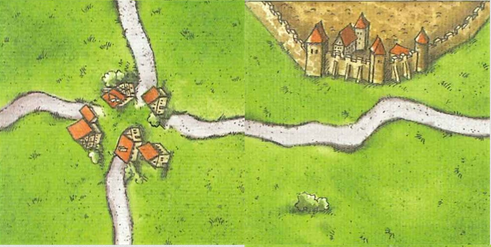
\includegraphics[width=0.8\textwidth]{images/tile125.png}
    \caption{deux tuiles du plateau}
    \label{two tiles}
\end{figure}
\subsubsection{Bords du plateau et graphe}
Même si le plateau est représenté par un tableau, il est initialement rempli de tuiles vides. Au fur et à mesure que la partie progresse, des tuiles sont ajoutées au plateau. C'est pourquoi il est nécessaire d'ajouter un champ \textbf{size} qui indique le nombre de tuiles jouées pendant la partie.\\

Pour déterminer les positions disponibles afin de poser une tuile sur le plateau, il faut d'abord identifier les positions sur le bord du plateau. Deux méthodes sont possibles :
\begin{itemize}
    \item À chaque fois qu'on veut jouer une tuile, on exécute une boucle qui recherche les positions sur le bord du plateau.
    \item On stocke les positions sur le bord du plateau dans une liste chaînée et à chaque fois, de nouvelles positions sont ajoutées à cette liste. 
\end{itemize}
En comparant les deux méthodes et compte tenu de la nature du jeu qui nécessite de jouer 72 tuiles, il est évident que la première méthode pourrait entraîner une complexité en temps considérable. Par conséquent, il est préférable d'utiliser la deuxième méthode, qui consiste à stocker les positions sur le bord du plateau dans une liste chaînée. 
On ajoute aussi  un autre champ graphe qui représente le graphe du plateau (il est détaillé dans la partie suivante),qui sert à calculer les composantes connexes afin de calculer le score.\\

Finalement la structure adoptée pour le plateau est la suivante :
\[
\text{struct board\_t} \left\{
\begin{array}{l}
\text{tiles} \quad \rightarrow \quad \text{un tableau de type struct tile\_t }\\
\text{size} \quad \rightarrow \quad \text{entier indiquant le nombre de tuile jouées}\\
\text{graph} \quad \rightarrow \quad \text{graphe de igraph }\\
\text{empty} \quad \rightarrow \quad \text{une liste chaînée de type struct tile\_t  }\\
\end{array}
\right.
\]
\subsection{Principales algorithmes du plateau}
Le plateau contient trois types de  fonctions:
\begin{itemize}
    \item \textbf{fonctions d'initialisation} : ces fonctions ont pour but d'allouer la mémoire pour le plateau, et de l'initialiser en ajoutant la coordonnée (0,0) au champ \textbf{empty} du plateau . Exemples: \textbf{Initialize\_board,Allocate\_board}.
    \item \textbf{fonctions de gestion de tuiles} :Ces fonctions permettent principalement d'ajouter les tuiles au plateau et de chercher une position valide pour chaque tuile. Exemples: \textbf{correct\_pasting, add\_tile, is\_corrected\_played}.
    \item \textbf{fonctions de gestion de empty} : ces fonctions garantissent l'ajout des nouvelles positions du bords du plateau ainsi que la suppression des positions occupées et le changement des identifiants des voisines de chaque tuile. Exemple:\textbf{ change\_neighbors}.
\end{itemize}
\subsubsection{Compléxité des alogrithmes}
soient N la taille de la structure \textit{board\_t} et \footnotesize {EMPTY\_SIZE} la taille de \textbf{empty}.
\begin{itemize}
    \item Les fonctions d'initialisation :Les fonctions \textbf{allocate\_board} et \textbf{initialize\_board} ont une complexité linéaire en temps et en espace, soit O(N), puisqu'elles se limitent à allouer la mémoire et à initialiser le champ \textbf{empty} du plateau.
    \item Les fonctions de gestion de tuiles : La fonction \textbf{correct\_pasting} accède à un élément de \textbf{empty}, qui est une liste chaînée, et effectue quatre appels à la fonction \textbf{flip\_tile}, qui fait pivoter les tuiles. Par conséquent, sa complexité est O(\footnotesize{MAX\_CONNECTIONS + EMPTY\_SIZE}), où \footnotesize{MAX\_CONNECTIONS} représente la taille des deux tableaux d'une tuile.
    \item Les fonctions de gestion de empty: Les fonctions \textbf{change\_neighbors} et \textbf{get\_possible\_moves} ont une complexité linéaire en \footnotesize{EMPTY\_SIZE} car elles accèdent aux éléments de \textbf{empty} et en suppriment certains.
\end{itemize}
\section{Plateau de jeu}
\subsection{Tuiles}
En observant la forme des tuiles de Carcassonne,on peut remarquer que chaque tuile est caractériser par 13 positions Comme l’illustre la figure \ref{positions tuiles}, 3 sur chaque côté et une au centre:

\begin{figure}[h]
     \begin{minipage}{0.48\textwidth}
    \centering
    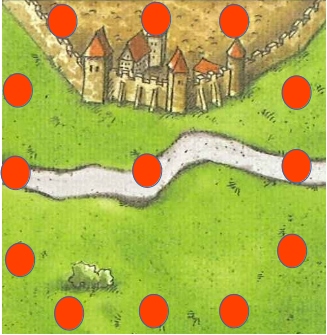
\includegraphics[width=0.6\textwidth,height=3.5cm]{images/tile1.png}
    \end{minipage}\hfill
    \begin{minipage}{0.48\textwidth}
    \centering
    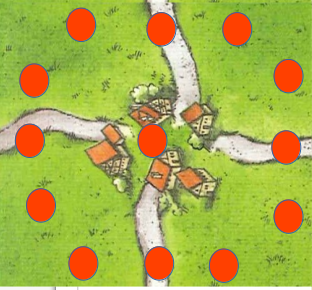
\includegraphics[width=0.6\textwidth,height=3.5cm]{images/tile2.png}
    \end{minipage}
    \caption{Les positions qui caractérisent les tuiles de Carcassonne}
    \label{positions tuiles}
\end{figure}
cela nous donne une idée pour définir une structure des tuiles. Comme le jeu contient un nombre fini d'objets (ville,route,champ,abbaye),on peut donc associer  à chaque objet une couleur. Par exemple,marron pour les villes,vert pour les champs,gris pour les routes...etc. Finalement toute tuile peut être représenté par la structure \textit{struct tile\_t} suivante:

\[
\text{struct tile\_t} \left\{
\begin{array}{l}
\text{t} \quad \rightarrow \quad \text{tableau d'entiers de taille 13}\\
\text{c} \quad \rightarrow \quad \text{tableau de couleurs de taille 13}\\
\end{array}
\right.
\]

\subsection{Pioche}
La pioche sera représentée par un type abstrait de données \textit{struct deck\_t}, dont l'implémentation dans le fichier deck.c contient trois champs:
\begin{itemize}
    \item deck qui un pointeur pointant sur les tuiles et qui sera alloué dynamiquement.
    \item size qui indique le nombre de tuiles stockées.
    \item capacity qui indique la taille de la mamoire allouée.
\end{itemize}
\[
\text{struct deck\_t} \left\{
\begin{array}{l}
\text{deck} \quad \rightarrow \quad \text{un poiteur pointant sur un tableau de tuiles }\\
\text{size} \quad \rightarrow \quad \text{entier}\\
\text{capacity} \quad \rightarrow \quad \text{entier}\\
\end{array}
\right.
\]
\subsection{Plateau}
\subsubsection{Plateau est un TAD }
Le plateau peut être implémenté de diverses façons, telles qu'une matrice ou une liste chaînée. Par conséquent, il est essentiel que la structure du Plateau soit un type abstrait de données, ce qui permet de rendre son implémentation plus flexible et indépendante du reste du code. \\
Pour représenter le plateau, une méthode simple consiste à utiliser une matrice de taille 2N, où N correspond au nombre total de tuiles. Cette approche offre plusieurs avantages, notamment un accès aux éléments du plateau en temps constant. Toutefois, cette méthode présente un inconvénient majeur : sa complexité en espace est de O($N^2$), ce qui est très coûteux en termes de mémoire.

Une deuxième méthode consiste à représenter le plateau par un tableau de taille N avec N le nombre de tuiles totales. Bien qu'il soit évident que cette méthode augmente la complexité en temps de certaines primitives, elle garantit une complexité linéaire en termes d'espace. Comme nous le verrons par la suite, la plupart des algorithmes associés à cette méthode sont linéaires, rendant cette approche plus envisageable.

Désormais, nous allons détailler la conception de la deuxième méthode.
\subsubsection{Tuiles dans le plateau}
\subsubsection*{Stockage des tuiles}
Stocker l'intégralité des tuiles dans le plateau augmenterait considérablement la complexité en espace. De plus, le nombre de tuiles différentes est fini. Par conséquent, nous pouvons stocker toutes les tuiles possibles dans un tableau \textbf{TILES\_TYPE}. Ainsi, nous pourrons stocker les tuiles dans le plateau en utilisant uniquement leurs indices dans \textbf{TILES\_TYPE}.
\subsubsection*{Rotation des tuiles}
Pendant la partie, la rotation des tuiles est autorisée. Il est donc nécessaire de savoir comment chaque tuile a été orientée. Pour ce faire, nous ajoutons un deuxième champ qui détermine l'orientation de la tuile sur le plateau.
\subsubsection*{Coordonnées et voisines d'une tuile}
Pour poser une tuile, il est nécessaire de connaître sa position aprés, ce qui rend indispensable l'ajout d'un champ déterminant cette position. Jusqu'à présent, le plateau présente un inconvénient majeur : pour passer d'une tuile à sa voisine, il faut parcourir à nouveau le tableau du plateau. Pour remédier à ce problème, nous pouvons ajouter des informations supplémentaires à chaque tuile concernant ses voisines en stockant leurs identifiants. Finalement les tuiles stockées dans le plateau vont avoir la stucture \textbf{struct status} suivante:
\[
\text{struct status} \left\{
\begin{array}{l}
\text{type\_id} \quad \rightarrow \quad \text{un entier indiquant le type de la tuile }\\
\text{rotation} \quad \rightarrow \quad \text{entier indiquant l'orientation de la tuile}\\
\text{x,y} \quad \rightarrow \quad \text{deux entiers indiquant les coordonnées }\\
\text{neighbors} \quad \rightarrow \quad \text{un tableau d'entier de taille 4  }\\
\end{array}
\right.
\]
Pour connaître précisément les identifiants de chaque voisine, il est nécessaire de les stocker de manière unique. Ainsi, chaque indice correspond à une direction spécifique. Nous choisissons respectivement les indices 0, 1, 2 et 3 pour représenter les directions nord, est, sud et ouest.\\
\textbf{Remarque}: Si une tuile ne possède pas de voisine dans une direction donnée, la valeur de cette voisine sera -1.
La figure \ref{two tiles} sera représenté par un tableau qui contient tile1 et tile2:
\begin{itemize}
    \item tile1=\{0,0,(0,0),{-1,-1,-1,1}\}
    \item tile2=\{1,0,(-1,0),{-1,0,-1,-1}\}
\end{itemize}
\begin{figure}[h]
    \centering
    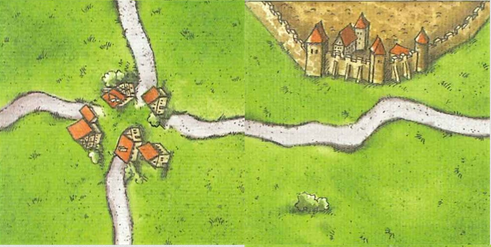
\includegraphics[width=0.8\textwidth]{images/tile125.png}
    \caption{deux tuiles du plateau}
    \label{two tiles}
\end{figure}
\subsubsection{Bords du plateau et graphe}
Même si le plateau est représenté par un tableau, il est initialement rempli de tuiles vides. Au fur et à mesure que la partie progresse, des tuiles sont ajoutées au plateau. C'est pourquoi il est nécessaire d'ajouter un champ \textbf{size} qui indique le nombre de tuiles jouées pendant la partie.\\

Pour déterminer les positions disponibles afin de poser une tuile sur le plateau, il faut d'abord identifier les positions sur le bord du plateau. Deux méthodes sont possibles :
\begin{itemize}
    \item À chaque fois qu'on veut jouer une tuile, on exécute une boucle qui recherche les positions sur le bord du plateau.
    \item On stocke les positions sur le bord du plateau dans une liste chaînée et à chaque fois, de nouvelles positions sont ajoutées à cette liste. 
\end{itemize}
En comparant les deux méthodes et compte tenu de la nature du jeu qui nécessite de jouer 72 tuiles, il est évident que la première méthode pourrait entraîner une complexité en temps considérable. Par conséquent, il est préférable d'utiliser la deuxième méthode, qui consiste à stocker les positions sur le bord du plateau dans une liste chaînée. 
On ajoute aussi  un autre champ graphe qui représente le graphe du plateau (il est détaillé dans la partie suivante),qui sert à calculer les composantes connexes afin de calculer le score.\\

Finalement la structure adoptée pour le plateau est la suivante :
\[
\text{struct board\_t} \left\{
\begin{array}{l}
\text{tiles} \quad \rightarrow \quad \text{un tableau de type struct tile\_t }\\
\text{size} \quad \rightarrow \quad \text{entier indiquant le nombre de tuile jouées}\\
\text{graph} \quad \rightarrow \quad \text{graphe de igraph }\\
\text{empty} \quad \rightarrow \quad \text{une liste chaînée de type struct tile\_t  }\\
\end{array}
\right.
\]
\subsection{Principales algorithmes du plateau}
Le plateau contient trois types de  fonctions:
\begin{itemize}
    \item \textbf{fonctions d'initialisation} : ces fonctions ont pour but d'allouer la mémoire pour le plateau, et de l'initialiser en ajoutant la coordonnée (0,0) au champ \textbf{empty} du plateau . Exemples: \textbf{Initialize\_board,Allocate\_board}.
    \item \textbf{fonctions de gestion de tuiles} :Ces fonctions permettent principalement d'ajouter les tuiles au plateau et de chercher une position valide pour chaque tuile. Exemples: \textbf{correct\_pasting, add\_tile, is\_corrected\_played}.
    \item \textbf{fonctions de gestion de empty} : ces fonctions garantissent l'ajout des nouvelles positions du bords du plateau ainsi que la suppression des positions occupées et le changement des identifiants des voisines de chaque tuile. Exemple:\textbf{ change\_neighbors}.
\end{itemize}
\subsubsection{Compléxité des alogrithmes}
soient N la taille de la structure \textit{board\_t} et \footnotesize {EMPTY\_SIZE} la taille de \textbf{empty}.
\begin{itemize}
    \item Les fonctions d'initialisation :Les fonctions \textbf{allocate\_board} et \textbf{initialize\_board} ont une complexité linéaire en temps et en espace, soit O(N), puisqu'elles se limitent à allouer la mémoire et à initialiser le champ \textbf{empty} du plateau.
    \item Les fonctions de gestion de tuiles : La fonction \textbf{correct\_pasting} accède à un élément de \textbf{empty}, qui est une liste chaînée, et effectue quatre appels à la fonction \textbf{flip\_tile}, qui fait pivoter les tuiles. Par conséquent, sa complexité est O(\footnotesize{MAX\_CONNECTIONS + EMPTY\_SIZE}), où \footnotesize{MAX\_CONNECTIONS} représente la taille des deux tableaux d'une tuile.
    \item Les fonctions de gestion de empty: Les fonctions \textbf{change\_neighbors} et \textbf{get\_possible\_moves} ont une complexité linéaire en \footnotesize{EMPTY\_SIZE} car elles accèdent aux éléments de \textbf{empty} et en suppriment certains.
\end{itemize}

\section{Implémentation des Graphes}

Un graphe, dans son sens mathématique courant, est une structure composée d'un ensemble de sommets, d'un ensemble de paires de sommets appelées arêtes, et d'un ensemble de valeurs associées à ces arêtes, appelées poids.\\
Il existe plusieurs classifications des graphes, parmi lesquelles l'une des plus importantes distingue les graphes orientés des graphes non orientés.\\
Un graphe orienté est un graphe où les arêtes ont une direction unique, tandis qu'un graphe non orienté est un graphe où chaque arête peut aller dans les deux sens.\\
\begin{figure}[h]
  \centering

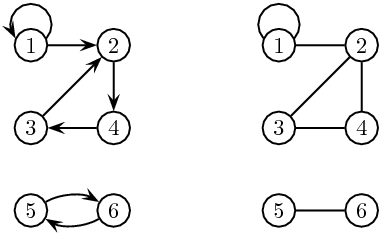
\includegraphics[width=10cm, height=6cm]{images/non_oriente.png}
\caption{À gauche un graphe orienté, à droite un graphe non orienté.}


\end{figure}\\
Un dessin d'un graphe est une représentation visuelle de l'objet mathématique ainsi défini. Un seul graphe peut posséder de multiples dessins. Un graphe planaire est une représentation de ce graphe dans laquelle les arêtes ne se croisent pas.\\
\begin{figure}[h]
    \centering
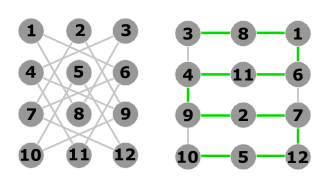
\includegraphics[width=10cm, height=6cm]{images/graphe_planaire.png}
\caption{à gauche, un graphe non planaire, à droite, un graphe planaire\\}
\end{figure}\\
\newpage
Une composante connexe d'un graphe non-orienté peut être définie comme un sous-graphe connecté qui n'est inclus dans aucun sous-graphe connecté plus grand.\\
\begin{figure}[ht]
    \centering
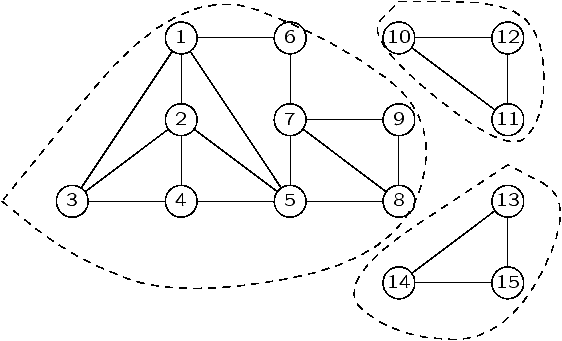
\includegraphics[width=10cm, height=6cm]{images/composantes_connexes.png}
\caption{Exemple des composantes connexes d'un graphe\\}
\end{figure}\\
Dans ce projet, nous avons choisi de manipuler des graphes non orientés en les représentant de manière planaire, car elles sont les structures les plus simples à manipuler.

\subsection{IGRAPH}
\subsubsection{Présentation}

La bibliothèque igraph est une bibliothèque offrant de nombreuses fonctions pour manipuler les graphes. Elle se distingue par sa capacité à gérer diverses classifications de graphes (comme les graphes orientés et non orientés), à prendre en charge plusieurs langages de programmation (tels que C et Python), et par sa simplicité d'utilisation (par exemple, pour l'ajout de sommets et d'arêtes).
 
Parmi les algorithmes disponibles dans igraph et prêts à être utilisés, on retrouve ceux dédiés aux plus courts chemins (comme A* et Dijkstra), aux parcours topologiques (tels que la profondeur et la largeur d'abord), au calcul des composantes connexes, ainsi que plusieurs autres.\\

\subsubsection{Types atomiques de IGRAPH}
Un type atomique dans igraph est un type de donnée de base utilisé pour représenter les éléments fondamentaux des graphes, tels que les sommets, les arêtes, et leurs attributs.\\
Les types atomiques de la bibliothèque igraph se distinguent par leur similitude avec les types usuels en C (int, float, etc.), tout en étant beaucoup plus simples à utiliser.\\
Parmi les types atomiques principaux de igraph, on distingue :

\begin{itemize}
    \item \texttt{igraph\_t} : le type atomique pour la structure de graphe.
    \item \texttt{igraph\_integer\_t} : le type atomique qui remplace les types \texttt{int} et \texttt{long int} de C, utilisé pour identifier les sommets.
    \item \texttt{igraph\_real\_t} : type similaire à \texttt{igraph\_integer\_t} mais pour les réels.
    \item \texttt{igraph\_vector\_t} : le type atomique pour une liste de nombres, avec plusieurs variantes telles que \texttt{igraph\_vector\_int\_t} pour manipuler les entiers.
    \item \texttt{igraph\_vector\_ptr\_t} : type similaire à \texttt{igraph\_vector\_t} mais stockant des pointeurs.
\end{itemize}

\subsubsection{fonctions de IGRAPH}

Parmi les principales fonctions d'igraph utilisées dans ce projet, on peut citer quelques-unes :

\begin{itemize}
    \item \texttt{igraph\_empty} : Cette fonction, fondamentale dans igraph, génère un graphe de type \texttt{igraph\_t} sans aucune arête entre les sommets générés.
    \item \texttt{igraph\_vcount} : Calcule le nombre de sommets dans le graphe.
    \item \texttt{igraph\_ecount} : Calcule le nombre d'arêtes dans le graphe.
    \item \texttt{igraph\_copy} : Cette fonction crée une copie d'un graphe.
    \item \texttt{igraph\_add\_vertices} : Ajoute de nouveaux sommets au graphe.
    \item \texttt{igraph\_add\_edge} : Ajoute une arête entre deux sommets.
    \item \texttt{igraph\_subcomponent} : Retourne la composante connexe à laquelle un sommet appartient.
    \item \texttt{igraph\_vector\_init} : Initialise un vecteur. Il existe plusieurs variantes comme \texttt{igraph\_vector\_int\_init} pour les entiers et \texttt{igraph\_vector\_ptr\_init} pour les pointeurs.
    \item \texttt{igraph\_vector\_destroy} : Libère la mémoire allouée par le vecteur. Il existe des variantes similaires à \texttt{igraph\_vector\_init}.
    \item \texttt{igraph\_destroy} : Libère la mémoire allouée par l'objet graphe.
\end{itemize}

\subsection{Les structures implémentés}
Dans l'implémentation de notre graphe pour ce projet, les attributs revêtent une importance cruciale dans la manipulation des sommets. Ils conservent des informations spécifiques sur chaque sommet du graphe en vue d'une utilisation ultérieure. La structure de ces attributs peut être définie comme suit :

\[
\text{attribute\_t} \left\{
\begin{array}{l}
\text{is\_there\_meeple} \quad \rightarrow \quad \text{tableau de 2 booléens}\\
\text{is\_merged} \quad \rightarrow \quad \text{booléen}\\
\text{color} \quad \rightarrow \quad \text{couleur}\\
\text{vertex\_is\_open} \quad \rightarrow \quad \text{booléen}\\
\text{coord} \quad \rightarrow \quad \text{coordonnées}\\ 
\text{already\_added\_to\_a\_component} \quad \rightarrow \quad \text{booléen}\\
\end{array}
\right.
\]


Le champ "\textbf{is\_merged}" indique si le sommet est fusionné ou non, même s'il apparaît non fusionné dans notre implémentation. Un sommet est considéré comme fusionné s'il fait partie d'une tuile qui vient d'être ajoutée et qui sera reliée à une autre tuile par une arête. Les tuiles fusionnées ne seront pas prises en compte lors du calcul des scores. Dans l'exemple suivant, les sommets 22, 23 et 24 sont fusionnés.\\
\begin{figure}[h]
    \centering
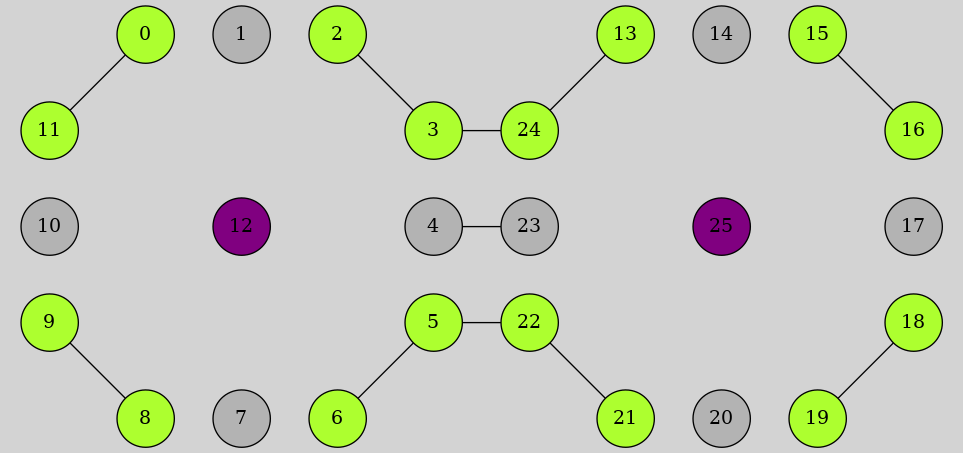
\includegraphics[width=0.8\textwidth, height=4cm]{images/fusionne.png}
\caption{Exemple de deux tuiles adjacentes\\}
\label{tuiles adjacentes}
\end{figure}

Au départ, nous avons ajouté cette structure parce que nous pensions qu'il était obligatoire de fusionner les sommets. Cependant, l'implémentation s'est avérée difficile, notamment en raison de la manipulation complexe des indices de graphe. Nous avons donc décidé de les séparer en ignorant l'un des sommets fusionnés lors du calcul des scores. Même après avoir réalisé qu'il n'était pas nécessaire de les séparer, nous avons choisi de conserver ce champ, car le calcul du score par le ladder fonctionne de cette manière.\\








Le champ \textbf{color} représente la couleur du nœud. Utile pour l'affichage du graphe et le calcul des scores\\





 Le champ \textbf{vertex\_is\_open} indique si l'ajout d'une tuile à une position précise permet d'ajouter une arête à ce nœud. Par exemple, dans la figure précédente, le nœud 10 est ouvert, tandis que les nœuds 4 et 12 sont fermés. Nous avons ajouté ce champ pour déterminer si l'ajout d'une tuile à une position donnée complète une structure. Au départ, nous avons essayé de définir pour chaque sommet les sommets situés aux extrémités de la composante représentée par ce sommet, mais cela s'est avéré très difficile car le nombre d'extrémités change constamment.





 
 
 
 Le champ \textbf{coord} indique les coordonnées des sommets, ce qui est utile uniquement pour l'affichage d'un graphe.\\ 

 
Le champ \textbf{already\_added\_to\_a\_component} précise si, lors du parcours d'une tuile, on est déjà passé par ce sommet en calculant la composante connexe d'un autre sommet. Par exemple, dans la figure \ref{tuiles adjacentes}, si l'on commence par le sommet 0 et calcule sa composante connexe, il n'est pas nécessaire de repasser par le sommet 11, car il appartient à la même composante connexe que 0, étant déjà traité dans la composante représentée par 0. Nous avons ajouté cette structure pour deux raisons : premièrement, elle réduit légèrement la complexité, et deuxièmement, elle résout les problèmes de calcul des scores que nous rencontrions auparavant. En effet, sans cette structure, une composante connexe calculée plusieurs fois pouvait augmenter le score de manière excessive.\\

Le champ "\textbf{is\_there\_meeple}" indique la présence d'un personnage sur le sommet qui l'a déposé.\\



 
 Dans toute la suite, un identifiant de tuile dans le graphe, généralement noté \textbf{id\_in\_graph} dans le projet, représente l'indice du premier sommet de cette tuile dans le graphe. Autrement dit, c'est l'indice de cette tuile dans la pioche multiplié par 13, cela permet de créer une bijection entre le plateau et le graphe, même si ces deux objets sont différents. Ainsi, la position d'une tuile sur le plateau est identifiée par les identifiants des tuiles adjacentes dans la pioche, stockés souvent dans un tableau appelé neighbours\_ids. Par exemple, pour ajouter une tuile dans l'exemple ci-dessous en position haut droite, cela signifie placer une tuile au-dessus de la tuile avec l'identifiant 0 dans la pioche et à gauche de la tuile avec l'identifiant 2 dans la pioche.
 
\begin{figure}[h]
    \centering
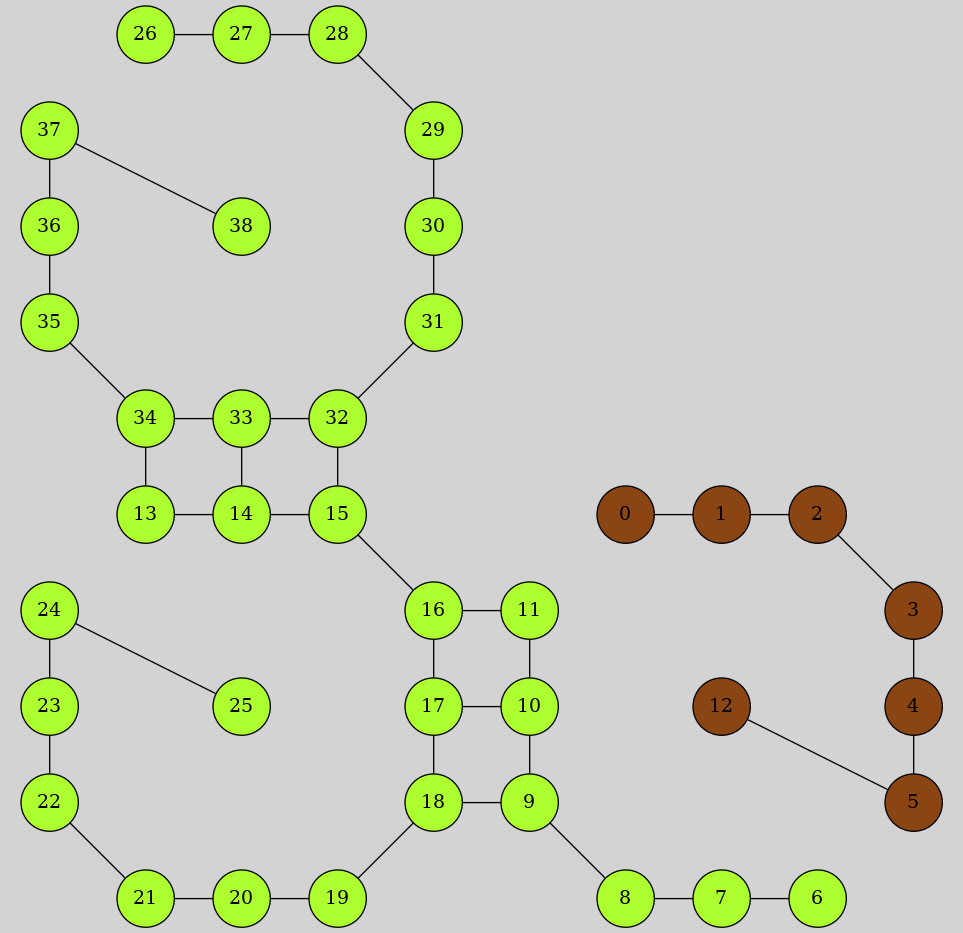
\includegraphics[width=10cm, height=10cm]{images/neighbours_ids.png}
\caption{Exemple des composantes connexes d'un graphe\\}
\end{figure}
Nous avons choisi cette implémentation après avoir essayé d'utiliser des coordonnées pour représenter les positions des tuiles dans le graphe. Cependant, cette méthode s'est avérée moins efficace, car il était nécessaire de déterminer les sommets adjacents aux sommets de chaque tuile en parcourant tous les sommets à chaque fois. En revanche, avec notre implémentation, nous pouvons accéder à ces sommets avec une complexité constante.

Pour stocker les attributs de tous les sommets, nous avons utilisé le tableau `attributes` de taille \(13 \times \text{NUM\_TILES}\). Nous avons choisi de ne pas allouer ce tableau dynamiquement après chaque ajout de tuile, car dans la majorité des cas, toutes les cartes de la pioche sont jouées. Ainsi, une allocation dynamique aboutirait à la même complexité en espace, mais avec un temps d'exécution beaucoup plus long.\\
 \subsection{Algorithmes implémentés}

 Pour simuler le jeu réel, nous avons utilisé plusieurs algorithmes pour manipuler les graphes. Ces algorithmes peuvent être classifiés en cinq sections décrites ci-dessous.
\subsubsection{Ajout d'une tuile}
\textbf{Problème :}

\textbf{Entrée :} Graphe de plateau + tuile à ajouter + position

\textbf{Score :} Ajouter la tuile au graphe à cette position\\
Pour coder l'action d'ajout d'une tuile à un graphe, nous avons utilisé les fonctions suivantes :

\begin{itemize}
    \item \texttt{create\_graph\_for\_tile}
        \item \texttt{add\_tile\_to\_graph}
\end{itemize}
La fonction \textbf{create\_graph\_for\_tile} ajoute des arêtes entre les sommets du graphe de la tuile qui vient d'être ajoutée au graphe du plateau. La fonction \textbf{add\_tile\_to\_graph} ajoute une tuile donnée à un graphe de plateau. Elle commence par ajouter 13 sommets au graphe du plateau, puis transforme ces 13 sommets en un sous-graphe représentant la tuile donnée en paramètre, en utilisant la fonction précédente. Ensuite, elle ajoute des arêtes entre les sommets de ce graphe de tuile et les sommets des graphes des tuiles adjacentes dans la représentation réelle du jeu.\\
Au départ, notre implémentation consistait à créer un graphe séparément pour chaque tuile, puis à les fusionner et à lier les arêtes. Cependant, pour une raison inconnue jusqu'à présent, cette méthode aboutissait à une faute de segmentation après l'ajout de cinq tuiles, due à la fonction \textbf{igraph\_disjoint\_union} de la bibliothèque igraph. Pour résoudre ce problème, nous avons décidé de remplacer cette fonction par \textbf{igraph\_add\_vertices}, ce qui a corrigé le problème. Nous avons également remarqué que cette dernière fonction a une complexité linéaire par rapport au nombre de sommets, tandis que \textbf{igraph\_disjoint\_union} a une complexité linéaire par rapport au nombre de sommets et d'arêtes.\\
Cet algorithme termine car il est de complexité linéaire par rapport au nombre de sommets et d'arêtes, la fonction \textbf{igraph\_add\_edge} ayant cette complexité. La correction de cet algorithme découle directement de la correction des fonctions de la bibliothèque igraph et des tests effectués tout au long du projet.\\
Pour tester ces fonctions, nous nous sommes appuyés sur une méthode d'affichage. L'implémentation de cet affichage sera abordée plus tard.\\
\subsubsection{Calcul de scores}
\textbf{Problème :}

\textbf{Entrée :} Graphe de plateau + tuile à ajouter + position

\textbf{Score :} Score ajouté si la tuile est ajoutée à cette position dans le graphe\\

Pour répondre à ce problème, nous avons principalement utilisé les fonctions suivantes :
\begin{itemize}
    \item \texttt{does\_adding\_ends\_a\_certain\_component}
    \item \texttt{set\_of\_new\_finished\_components\_after\_adding}
    \item \texttt{calculate\_score\_in\_a\_component}
    \item \texttt{added\_score}
\end{itemize}
La fonction \textbf{does\_adding\_ends\_a\_certain\_component} prend en entrée un graphe pour le plateau, un identifiant de tuile dans le graphe supposée être placée récemment sur le plateau, ainsi qu'un sommet sur la tuile. Cette fonction répond à la question suivante : est-ce que la composante connexe représentée par ce sommet est terminée ou non ? Pour cela, elle utilise la fonction subcomponent de la bibliothèque igraph, qui calcule directement la composante connexe à laquelle appartient ce sommet. Ensuite, la fonction vérifie s'il existe un sommet ouvert dans cette composante. Si elle en trouve un, alors la composante n'est pas terminée ; sinon, la structure est considérée comme terminée. La terminaison de cet algorithme est garantie car il a la même complexité que subcomponent, qui est linéaire par rapport au nombre de sommets et d'arêtes. La correction de cet algorithme découle de la simple proposition selon laquelle "une composante connexe est terminée si tous ses sommets sont fermés".\\
La fonction \textbf{set\_of\_new\_finished\_components\_after\_adding}\\ prend en paramètres un graphe de plateau, une tuile non encore déposée et son identifiant dans la pioche, ainsi que la position où l'on souhaite déposer la tuile. Elle répond à la question suivante : si l'on dépose une tuile à une certaine position, cela va-t-il terminer une structure du graphe ou non ? Et si oui, lesquelles ?\\

La fonction parcourt les sommets de la tuile en rassemblant les composantes connexes qui seront terminées si l'on pose la tuile à cette position, tout en veillant à ne pas ajouter la même composante deux fois.\\
La complexité de cette fonction est similaire à celle de la fonction \\\textbf{does\_adding\_ends\_a\_certain\_component}, et donc de l'ordre du nombre de sommets et d'arêtes, ce qui garantit sa terminaison. De plus, la correction de cette fonction découle également de la correction de la fonction \\\textbf{does\_adding\_ends\_a\_certain\_component}.\\

La fonction \textbf{added\_score} prend en paramètres un graphe représentant un plateau, une position, une tuile et son identifiant dans la pioche, et calcule le score ajouté si l'on place la tuile dans cette position du graphe. Elle boucle sur les composantes terminées retournées par la fonction précédente et calcule le score de chacune d'elles à l'aide de la fonction \textbf{calculate\_score\_in\_a\_component}, qui détermine le score dans une composante connexe. La complexité de cette fonction est similaire à celle de la fonction précédente, et sa terminaison découle également de celle-ci.\\
La réflexion derrière tout cela découle directement de l'ajout du champ décisionnel déterminant si un sommet est ouvert ou fermé, ainsi que de la proposition précédemment évoquée qui établit le lien entre les sommets fermés et la terminaison des composantes connexes. Cependant, nous avons rencontré des problèmes initialement car nous n'avons pas remarqué la fonction subcomponent parmi les fonctions disponibles dans la bibliothèque igraph, en raison de la difficulté de recherche dans celle-ci.Au début, nous avons travaillé avec la fonction \textbf{connected\_components} qui répond à nos besoins, mais cela necissite beaucoup d'efforts.\\

Pour tester ces fonctions, nous avons tenté d'ajouter les tuiles dans des positions dont nous connaissions les valeurs de retour, puis nous les avons principalement testées à l'aide d'instructions assert.
\\

\subsubsection{fonctions aidant à manipuler les stratégies}
Même si nous allons réserver une autre section pour discuter des stratégies des joueurs, nous avons décidé d'intégrer ici deux fonctions qui aideront à manipuler ces stratégies, car elles ne seront pas présentes dans aucun fichier des joueurs. Ces fonctions sont :
\begin{itemize}
    \item \texttt{number\_of\_vertices\_in\_new\_component}
    \item \texttt{get\_biggest\_component\_of\_player\_in\_a\_position}
\end{itemize}
La fonction \texttt{number\_of\_vertices\_in\_new\_component} prend en paramètre un graphe de plateau, une tuile et son identifiant dans la pioche, une position et un sommet de cette tuile. Cette fonction calcule le nombre de sommets dans la composante représentée par ce sommet si la tuile est placée à cette positions dans le plateau de graphe.\\

La fonction \texttt{get\_biggest\_component\_of\_player\_in\_a\_position} prend \\en paramètre un graphe de plateau, une tuile et son identifiant, la position où l'on souhaite poser cette tuile, une couleur, un mode, et un nombre de personnages. Elle calcule la plus grande composante connexe terminée de la couleur spécifiée si la tuile est placée à cette position. Ensuite, selon des critères susceptibles de varier en fonction des stratégies des joueurs, elle retourne la composante correspondante.\\

La complexité en temps des deux fonctions est linéaire par rapport au nombre de sommets et d'arêtes. La terminaison est garantie puisqu'elles utilisent des fonctions dont nous avons démontré la terminaison. La correction est assurée par les tests : nous avons utilisé une combinaison de tests assert et d'affichage pour les vérifier.













\subsubsection{Manipulation des personnages}


\textbf{Problème :}

\textbf{Entrée :} Graphe de plateau + ensemble des personnages + identifiants des joueurs

\textbf{Sortie :} Manipulation des personnages par le joueur\\
pour repondre à ce probleme on a essayé d'implémenter plusieurs fonctions :
\begin{itemize}
\item \texttt{meeple\_can\_be\_added}
\item \texttt{which\_player\_has\_more\_meeples\_in\_component}
\item \texttt{add\_meeple}
\item \texttt{retrieve\_meeples}
\end{itemize}

La fonction \texttt{meeple\_can\_be\_added} décide si un personnage peut être placé ou non dans un sommet donné. Un personnage peut être placé dans un sommet si la composante connexe représentée par ce sommet ne contient pas déjà de personnage, et si la tuile à laquelle ce sommet appartient ne contient pas non plus de personnage. Nous avons vérifié la correction et la terminaison de cette fonction par le biais de tests. Au départ, nous avons cherché à obtenir une complexité constante, c'est pourquoi nous avons essayé d'ajouter un champ \texttt{there\_is\_meeple} à la structure des attributs. Ce champ change chaque fois qu'un personnage est ajouté de la manière suivante : si un personnage est ajouté sur un sommet, nous mettons \texttt{there\_is\_meeple} à 1 pour tous les sommets appartenant à la même composante connexe ainsi que pour les sommets appartenant à la même tuile. Cependant, cette approche a rendu le code un peu moins élégant et nous avons rencontré des résultats inattendus lors des tests.\\
La fonction \texttt{which\_player\_has\_more\_meeples\_in\_component} calcule le nombre de personnages de chaque joueur dans une structure et retourne l'identifiant du joueur qui possède le plus de personnages. Au début, nous avons mal interprété le sujet en pensant qu'il ne pouvait y avoir qu'un seul personnage dans la structure, mais nous avons corrigé cette erreur par la suite en ajoutant cette fonction.

La fonction \texttt{retrieve\_meeples} permet de récupérer les personnages déjà placés et retourne le nombre de personnages récupérés par un joueur dont l'identifiant est donné en paramètre.\\

Toutes les fonctions mentionnées ont une complexité linéaire par rapport au nombre de sommets et d'arêtes\\

Les tests pour cette partie ont principalement été réalisés par visualisation. Un sommet contenant un personnage du joueur ayant l'identifiant 0 est coloré en rouge, tandis que celui du joueur 1 est coloré en bleu. Les sommets sans personnage, mais où il est impossible de placer un personnage, sont colorés en blanc. La figure ci-dessous illustre un exemple de ces tests où le joueur d'identifiant 1 a posé un personnage dans le sommet indicé 4.\\
\begin{figure}[h]
    \centering
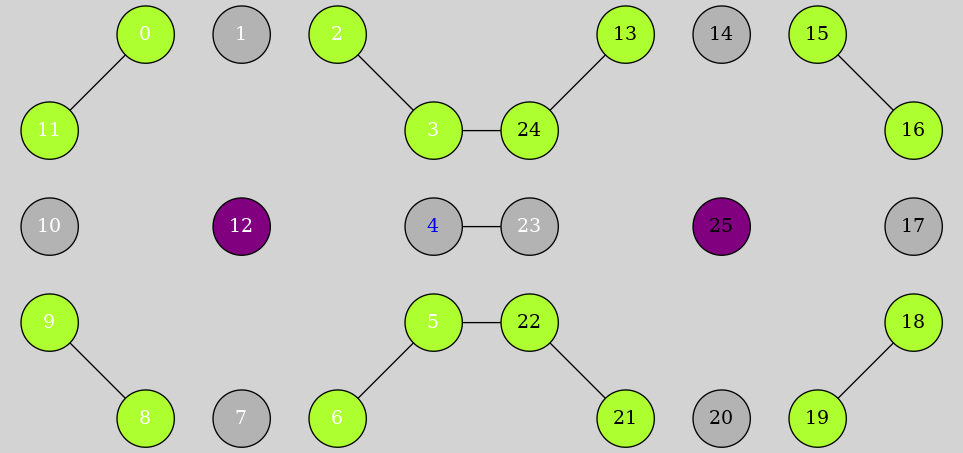
\includegraphics[width=10cm, height=5cm]{images/meeples.png}
\caption{Exemple des composantes connexes d'un graphe\\}



\end{figure}
\subsubsection{Affichage}

Pour nous aider à déboguer et effectuer des tests, nous avons écrit une fonction \texttt{display\_graph} qui génère un fichier avec un nom donné en paramètre, au format .dot. À partir d'un graphe fourni en paramètre, cette fonction remplit le fichier avec les données du graphe de manière à ce qu'elles soient interprétables par le langage dot, elle est de complexité linéaire en nombre d'arêtes et sommets




\section{Joueurs}
Dans notre implémentation du jeu Carcassonne, seulement deux joueurs peuvent jouer à la fois. Chacun d'eux possède une vision et des stratégies de jeu qui diffèrent de l'autre, et qui varient également selon le mode de jeu. Ainsi, on peut formuler le problème suivant :

\textbf{Problème :}
\begin{itemize}
\item \textbf{Entrée :} joueur + mode
\item \textbf{Sortie :} stratégies
\end{itemize}
Les deux joueurs utilisent une grande partie du même code, qui est regroupée dans le fichier \textbf{src/playerStruc.h}. Ce fichier contient principalement les éléments partagés entre les deux joueurs, notamment la définition de la structure de joueur, qui est la suivante :


\[
\text{player\_t} \left\{
\begin{array}{l}
\text{player\_id} \quad \rightarrow \quad \text{entier}\\
\text{myboard} \quad \rightarrow \quad \text{plateau}\\
\text{config} \quad \rightarrow \quad \text{configuration de jeu}\\
\text{name} \quad \rightarrow \quad \text{nom de joueur}\\ 
\end{array}
\right.
\]

Nous avons opté pour cette structure car les joueurs sont initialisés par le serveur à l'aide des trois premiers champs. Le quatrième champ est utilisé pour distinguer les deux joueurs, ce qui permet à l'exécuteur de savoir quel joueur a joué un coup.\\

Ce fichier contient aussi une fonction appelée \textbf{update\_player\_board}, qui ajoute des tuiles et des personnages au plateau du joueur. De plus, cette fonction permet au joueur de récupérer ses personnages lorsqu'une structure est terminée.

\subsection{Joueur naïf}
Le premier joueur est considéré comme naïf et ne possède aucune stratégie. Sa seule tactique consiste à chercher la première position possible, assurée par la fonction \\get\_possible\_moves dans l'implémentation du plateau. Il ne tourne même pas les tuiles, ne connaît pas les personnages, et donc ne les utilise pas. Ainsi, les trois modes de jeu sont identiques pour lui.



\subsection{Joueur intélligent}

Ce joueur possède des stratégies qui diffèrent d'un mode à l'autre. Mais en général, il utilise les fonctions suivantes définies dans le fichier \textbf{player\_functions.h} :

\begin{itemize}
    \item \texttt{get\_optimal\_position\_no\_meeple}
    \item \texttt{get\_biggest\_open\_component}
    \item \texttt{get\_biggest\_finished\_component}
    \item \texttt{get\_a\_position\_where\_there\_is\_no\_meeple}
    \item \texttt{get\_random\_possible\_position}
\end{itemize}
Toutes ces fonctions itèrent sur les positions possibles en retournant chaque fois la carte dans les quatre orientations possibles. Ces algorithmes se terminent tous car ils utilisent des fonctions dont nous avons prouvé la terminaison auparavant, et ils sont tous corrects car ils utilisent des algorithmes de force brute.

La fonction \texttt{get\_optimal\_position\_no\_meeple} itère en renvoyant la position qui donne le meilleur score selon la fonction \texttt{added\_score} précédemment définie.

La fonction \texttt{get\_biggest\_open\_component} itère sur les positions possibles et renvoie celle caractérisée par la plus grande composante connexe ouverte de la même couleur que celle en entrée, tout en satisfaisant des contraintes spécifiques propres à chaque mode de jeu.

La fonction \texttt{get\_biggest\_finished\_component} itère sur les positions possibles et choisit la plus grande structure pour une couleur donnée en paramètre qui peut être complétée en ajoutant la tuile que le joueur possède.

La fonction \texttt{get\_a\_position\_where\_there\_is\_no\_meeple} itère également et renvoie la première position où le joueur peut déposer un personnage.

La fonction \texttt{get\_random\_possible
position} renvoie la première position possible si elle existe, sinon elle retourne une position aléatoire qui entraîne la défaite du joueur.

Nous avons choisi d'implémenter ces fonctions car elles semblent être parmi les premières choses auxquelles un joueur réel penserait s'il veut jouer à un tel jeu.

En raison des contraintes temporelles, nous n'avons pas pu effectuer des tests approfondis sur ces fonctions. Nous les avons seulement testées en plaçant des tuiles dans des positions données par ces fonctions, puis en vérifiant visuellement à chaque fois à l'aide d'une représentation graphique qu'elles respectent bien nos attentes.
La complexité de ces fonctions, à l'exception de la dernière, est égale à la complexité de la fonction \textbf{get\_possible\_moves} multipliée par \textbf{NUM\_TILES}, et pour la dernière fonction, la complexité est la même que celle de \textbf{get\_possible\_moves}.

ces fonction sont utilisés dans les stratégies ensuite par le joueur pour définir les trois modes :

\subsubsection{Mode sans personnage}
Dans ce mode, le joueur tente d'abord de placer la tuile à l'emplacement qui rapporte le plus de points. Si plusieurs emplacements maximaux sont trouvés, il choisit le premier. S'il ne trouve aucune position possible, il en choisit une aléatoirement. L'algorithme est le suivant :
\begin{algorithm}[H]
\caption{play\_in\_no\_meeple}
\begin{algorithmic}[1]
\STATE \textbf{Input:} board, t, player\_id
\STATE \textbf{Output:} optimal position
\STATE Initialize config $\gets$ \{mode = NO\_MEEPLE, meeples = , deck = player.config.deck\}
\STATE optimal $\gets$ \textsc{get\_optimal\_position\_no\_meeple}(board, t, player\_id)
\IF{optimal $\neq$ NULL}
    \RETURN optimal
\ENDIF
\STATE optimal $\gets$ \textsc{get\_biggest\_open\_component}(board, t, player\_id, config, GRAY)
\IF{optimal $\neq$ NULL}
    \RETURN optimal
\ENDIF
\STATE optimal $\gets$ \textsc{get\_random\_possible\_position}(board, t, player\_id)
\RETURN optimal
\end{algorithmic}
\end{algorithm}

\subsubsection{Mode à personnages infini}

Dans ce mode, le joueur tente d'abord de terminer les composantes connexes marron, car elles rapportent le plus de points et il craint que l'autre joueur les termine avant lui. S'il n'y parvient pas, il essaie soit de bloquer l'adversaire en fermant la plus grande composante connexe de route appartenant à celui-ci, car il pense que ces composantes se développent rapidement et que chaque sommet de route rapporte 4 points à l'adversaire, soit il cherche une position où il peut poser un personnage, car il considère qu'ayant un nombre infini de personnages, il vaut mieux en placer un à chaque tour. Enfin, s'il ne trouve aucune option viable, il choisit une position correcte aléatoire pour poser la tuile, et s'il n'en trouve pas, il la pose n'importe où et échoue. L'algorithme peut être défini comme suit :

\begin{algorithm}[H]
\caption{play\_in\_infinite\_meeple}
\begin{algorithmic}[1]
\STATE \textbf{function} play\_in\_infinite\_meeple(board, t, player\_id)
    \STATE config $\gets$ \{mode: INFINITE\_MEEPLE, meeples: meeples, deck: player.config.deck\}
    \STATE brown $\gets$ get\_biggest\_finished\_component(board, t, player\_id, BROWN, config)
    \IF {brown $\neq$ \textbf{NULL}}
        \RETURN brown
    \ENDIF
    \IF {rand() \% 2 == 0}
        \STATE road\_adversary $\gets$ get\_biggest\_finished\_component(board, t, 1 - player\_id, GRAY, config)
        \IF {road\_adversary $\neq$ \textbf{NULL}}
            \RETURN road\_adversary
        \ENDIF
    \ELSE
        \STATE no\_meeple $\gets$ get\_a\_position\_where\_there\_is\_no\_meeple(board, t, player\_id)
        \IF {no\_meeple $\neq$ \textbf{NULL}}
            \RETURN no\_meeple
        \ENDIF
    \ENDIF
    \STATE random $\gets$ get\_random\_possible\_position(board, t, player\_id)
    \RETURN random
\STATE \textbf{end function}
\end{algorithmic}
\end{algorithm}\subsubsection{Mode à personnages fini}

Ce mode est similaire aux modes de personnages infinis, mais il diffère dans l'avant-dernière étape. En effet, le joueur considère désormais les personnages comme précieux et doit les utiliser avec prudence. À partir de ce moment, 
 il estime qu'il est inutile de placer des personnages sur les sommets de champs, car ces derniers ne rapportent beaucoup de points que lorsqu'ils sont nombreux, et la structure de champ devient très difficile à terminer lorsqu'elle est grande. De plus, il évite de poser des personnages sur les structures marron, car elles se terminent généralement en un seul coup. Il reste donc uniquement les structures de route. Le joueur place sa carte sur la plus grande composante de route ouverte et y pose un personnage s'il en a plus d'un.

\begin{algorithm}[H]
\caption{play\_in\_finite\_meeple}
\begin{algorithmic}[1]
\STATE \textbf{function} play\_in\_finite\_meeple(board, t, player\_id, config)
    \STATE brown $\gets$ get\_biggest\_finished\_component(board, t, player\_id, BROWN, config)
    \IF {brown $\neq$ \textbf{NULL}}
        \RETURN brown
    \ENDIF
    \IF {rand() \% 2 == 0}
        \STATE road\_adversary $\gets$ get\_biggest\_finished\_component(board, t, 1-player\_id, GRAY, config)
        \IF {road\_adversary $\neq$ \textbf{NULL}}
            \RETURN road\_adversary
        \ENDIF
    \ELSE
        \STATE open\_road\_meeple $\gets$ get\_biggest\_open\_component(board, t, player\_id, config, GRAY)
        \IF {open\_road\_meeple $\neq$ \textbf{NULL}}
            \RETURN open\_road\_meeple
        \ENDIF
    \ENDIF
    \STATE random $\gets$ get\_random\_possible\_position(board, t, player\_id)
    \RETURN random
\STATE \textbf{end function}
\end{algorithmic}
\end{algorithm}

La terminaison et la correction de ces fonctions sont garanties par les fonctions qu'elles utilisent, dont nous avons déjà démontré la correction et la terminaison. Les complexités de ces fonctions sont égales aux complexités des fonctions les plus coûteuses qu'elles appellent. Ainsi, ces complexités sont toutes équivalentes à celle de la fonction \texttt{get\_possible\_moves} multipliée par \texttt{NUM\_TILES}.

Nous avons testé ces algorithmes sur le serveur. En général, ils répondent aux attentes. Par exemple, une visualisation graphique en mode fini montre clairement que le joueur privilégie toujours la terminaison des composantes marrons avant de placer ses personnages uniquement dans les composantes des routes longues.







































\section*{Conclusion}
En conclusion, ce projet nous a permis d'acquérir de nouvelles compétences techniques, collaboratives et intellectuelles. Nous avons désormais une compréhension claire de nombreuses notions qui semblaient ambiguës avant le projet, telles que les bibliothèques statiques et dynamiques, leur manipulation, et l'utilisation de gcov. Cependant, plusieurs éléments que nous souhaitions réaliser n'ont pas été complétés, comme l'intégration de clang, la documentation avec doxygen, et la création d'un README soigné, des tâches que nous avions accomplies dans le cours de programmation impérative 2 mais que nous n'avons pas pu finaliser ici en raison d'une mauvaise gestion du temps. L'une des difficultés rencontrées au début du projet concernait la représentation des structures importantes, mais nous avons réussi à surmonter cet obstacle par la suite.

\end{document}

